\documentclass[12pt]{article}
\usepackage[english]{babel}
\usepackage[utf8x]{inputenc}
\usepackage{amsmath}
\usepackage{graphicx}
\usepackage[a4paper]{geometry}

\begin{document}
\begin{titlepage}

% definition of custom command for horizontal lines
\newcommand{\HRule}{\rule{\linewidth}{0.5mm}}

\center
% HEADING
\textsc{\LARGE University of Dublin,\\Trinity College}\\[1.0cm]

\includegraphics[width=0.2\textwidth]{logo.png}

\HRule \\[0.4cm]
\textsc{\Large JS Engineering: 3C2 Digital Circuits}\\[0.25cm]
\textsc{\large D2: The MOS/CMOS Inverter}\\[0.1cm]
\HRule \\[0.4cm]
 
% AUTHORS
\begin{minipage}{0.5\textwidth}
\begin{flushleft} \large
\emph{Author:}
\\Edmond \textsc{O'Flynn} 12304742
\end{flushleft}
\end{minipage}
~
\begin{minipage}{0.4\textwidth}
\begin{flushleft} 
\large
\emph{Demonstrator:} \\
Cormac \textsc{Molloy} 
\end{flushleft}
\end{minipage}\\[3cm]

% DATE
{\large \today}\\[2cm] 

% LOGO
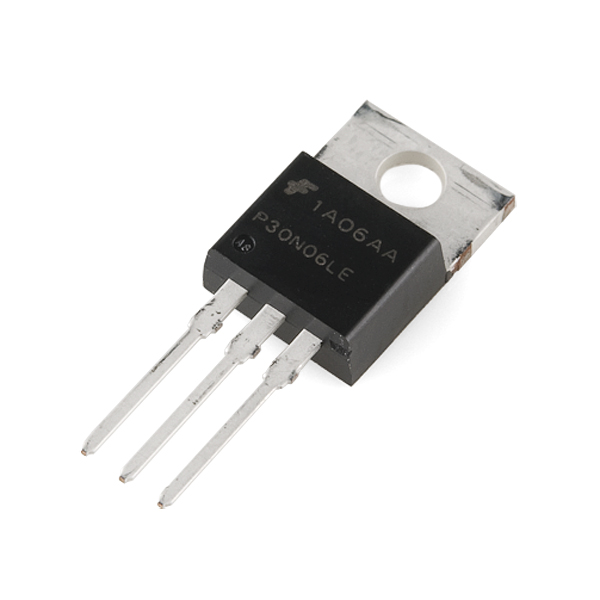
\includegraphics[width=0.2\textwidth]{mosfet.jpg}
\clearpage
\end{titlepage}

\newgeometry{top=2cm,left=2cm,bottom=2cm,right=2cm}

\tableofcontents
\thispagestyle{empty}
\cleardoublepage
\setcounter{page}{1}

\section{Abstract}
Lab D2 introduces the concept of MOS transistor simulation in the MultiSim 13.0 environment, and theory associated with the static and dynamic characteristics which show the effect of performance in various environments in the modern world of technology.
\section{Introduction}
The aim for this lab is to show and understand the differences between \emph{n-channel} and \emph{p-channel} MOS transistors, to test various properties of MOS, and also to demonstrate the performance of CMOS inverters. These states are modelled and examined during this laboratory through adjusting and viewing the properties associated with these states within circuit design.
\section{Theory}
\subsection{What is a MOSFET?}
MOSFETs are used in modern day technology to control electronics, similarly to a BJT. However a BJT controls by current, while a MOSFET is a voltage-controlled device that acts like a variable resistor, where voltage applied changes how the device conducts within the circuit. MOSFETs have a very high impedance, therefore it's extremely easy to drive on low current.
\subsection{How does a MOSFET work?}
A MOSFET is a voltage controlled field effect transistor that has its gate electrode highly insulated from the semiconductor in the transistor by a very thin layer of insulating material. The insulated metal gate acts similarly to how a capacitor's plate which causes an extremely high input resistance due to isolation. However, when a voltage is applied to the gate, the width of the \emph{drain-source} channel changes, and the device conducts freely.
\subsection{Abbreviations}
\begin{itemize}
\item MOSFET
\begin{itemize}
\item MOSFET stands for \emph{Metal-Oxide Semiconductor Field Effect Transistor}, and is used to amplify signals or act as a switch in an electronic circuit. Their main advantage is the low current required (1mA) in order to activate, while delivering a much higher current load (10-50A).
\end{itemize}
\item N-channel
\begin{itemize}
\item An n-channel MOS transistor is classified as a semiconductor device where the electrons control the current flowing through it by utilising three terminal substrates: \emph{gate}, \emph{drain} and \emph{source}. These terminals allow for three different modes of operation that affect the output differently, whose modes are \emph{cut-off}, \emph{triode}, and \emph{saturation}. The n-channel generally has a lower resistance than a p-type MOS transistor. 
\end{itemize}
\item P-channel
\begin{itemize}
\item A p-type MOS transistor pertains to the same properties in terms of operation as a n-type MOS transistor, where the differences lie in its substrate composition, where the charge characteristics are holes instead of electrons.
\end{itemize}
\item Gate
\begin{itemize}
\item 
\end{itemize}
\item Drain
\begin{itemize}
\item 
\end{itemize}
\item Source
\begin{itemize}
\item 
\end{itemize}
\item $V_{GS}$
\begin{itemize}
\item 
\end{itemize}
\item $V_T$
\begin{itemize}
\item 
\end{itemize}
\item $V_H$
\begin{itemize}
\item 
\end{itemize}
\item $V_{I}$
\begin{itemize}
\item 
\end{itemize}
\item $V_O$
\begin{itemize}
\item 
\end{itemize}
\item $V_{DD}$
\begin{itemize}
\item Positive power supply voltage
\end{itemize}
\item $V_L$
\begin{itemize}
\item 
\end{itemize}
\item $V_{IL MAX}$
\begin{itemize}
\item 
\end{itemize}
\item $V_{IH MIN}$
\begin{itemize}
\item 
\end{itemize}
\item $V_{OL}$
\begin{itemize}
\item 
\end{itemize}
\item $V_{OH}$
\begin{itemize}
\item 
\end{itemize}
\item $K_{n}$
\begin{itemize}
\item 
\end{itemize}
\item $R_{d}$
\begin{itemize}
\item Resistive load applied to the drain of the MOS transistor
\end{itemize}
\item $t_{PHL}$
\begin{itemize}
\item The propagation delay that exists for an input changing from a logic high to a logic low.
\end{itemize}
\item $t_{PLH}$
\begin{itemize}
\item The propagation delay that exists for an input changing from a logic low to a logic high.
\end{itemize}
\item $t_{f}$
\begin{itemize}
\item The time taken for the voltage to cross the transistor junction in forward active mode.
\end{itemize}
\item $t_{r}$
\begin{itemize}
\item The time taken for the voltage to cross the transistor junction in reverse active mode.
\end{itemize}
\end{itemize}
\section{MOS Transistor Characteristics}
Using MultiSim 13.0, the following schematic should be drawn and connected up.
\subsection{Procedure}
\begin{itemize}
\item Create a new page and insert a N-MOS transistor with the following values onto the design schematic sheet. Ensure to save them to the user database for easy access.
\begin{itemize}
\item Length: $1\cdot10^{-4}$m
\item Width: $2\cdot10^{-4}$m
\item V$_{TO}$: 1V
\item $K_n$: $2\cdot10^{-5}$A/V${^2}$
\end{itemize}
\item Later on for a P-MOS transistor, the following values should be used instead, which should be also saved in the user database to save time.
\begin{itemize}
\item Length: $1\cdot10^{-4}$m
\item Width: $2\cdot10^{-4}$m
\item V$_{TO}$: -1V
\item $K_p$: $2\cdot10^{-5}$A/V${^2}$
\end{itemize}
\item Set up the schematic as shown in the diagram
\item Ensure the components are wired up correctly, including the ground.
\item Place a probe looking towards the drain of the MOS transistor
\item Perform a sweep using $V_{DS}$ as source 1, and $V_{GS}$ as source 2.
\item Also make sure that I(Probe1) has been added to the list of selected variables for analysis for generating a plot of I$_D$ v V$_{GS}$
\item On sweeping this, change the value of the MOS transistor width to 4$\mu$m and rerun the analysis.
\end{itemize}
\subsection{Results}
\begin{table}[h]
\centering
\label{my-label}
\begin{tabular}{lll}
       & N-Channel                                     & P-Channel                                      \\
Length & 0.0001m                                       & 0.0001m                                        \\
Width  & 0.0001m                                       & 0.0001m                                        \\
$V_{TO}$    & 1V                                            & -1V                                            \\
$K_p$, $K_n$  & $2\cdot10^{-5}$ A/V$^{2}$ & $1\cdot10^{-5}$ A/V$^{2}$
\end{tabular}
\caption{Reference Values}
\end{table}
\begin{align*}
\centering
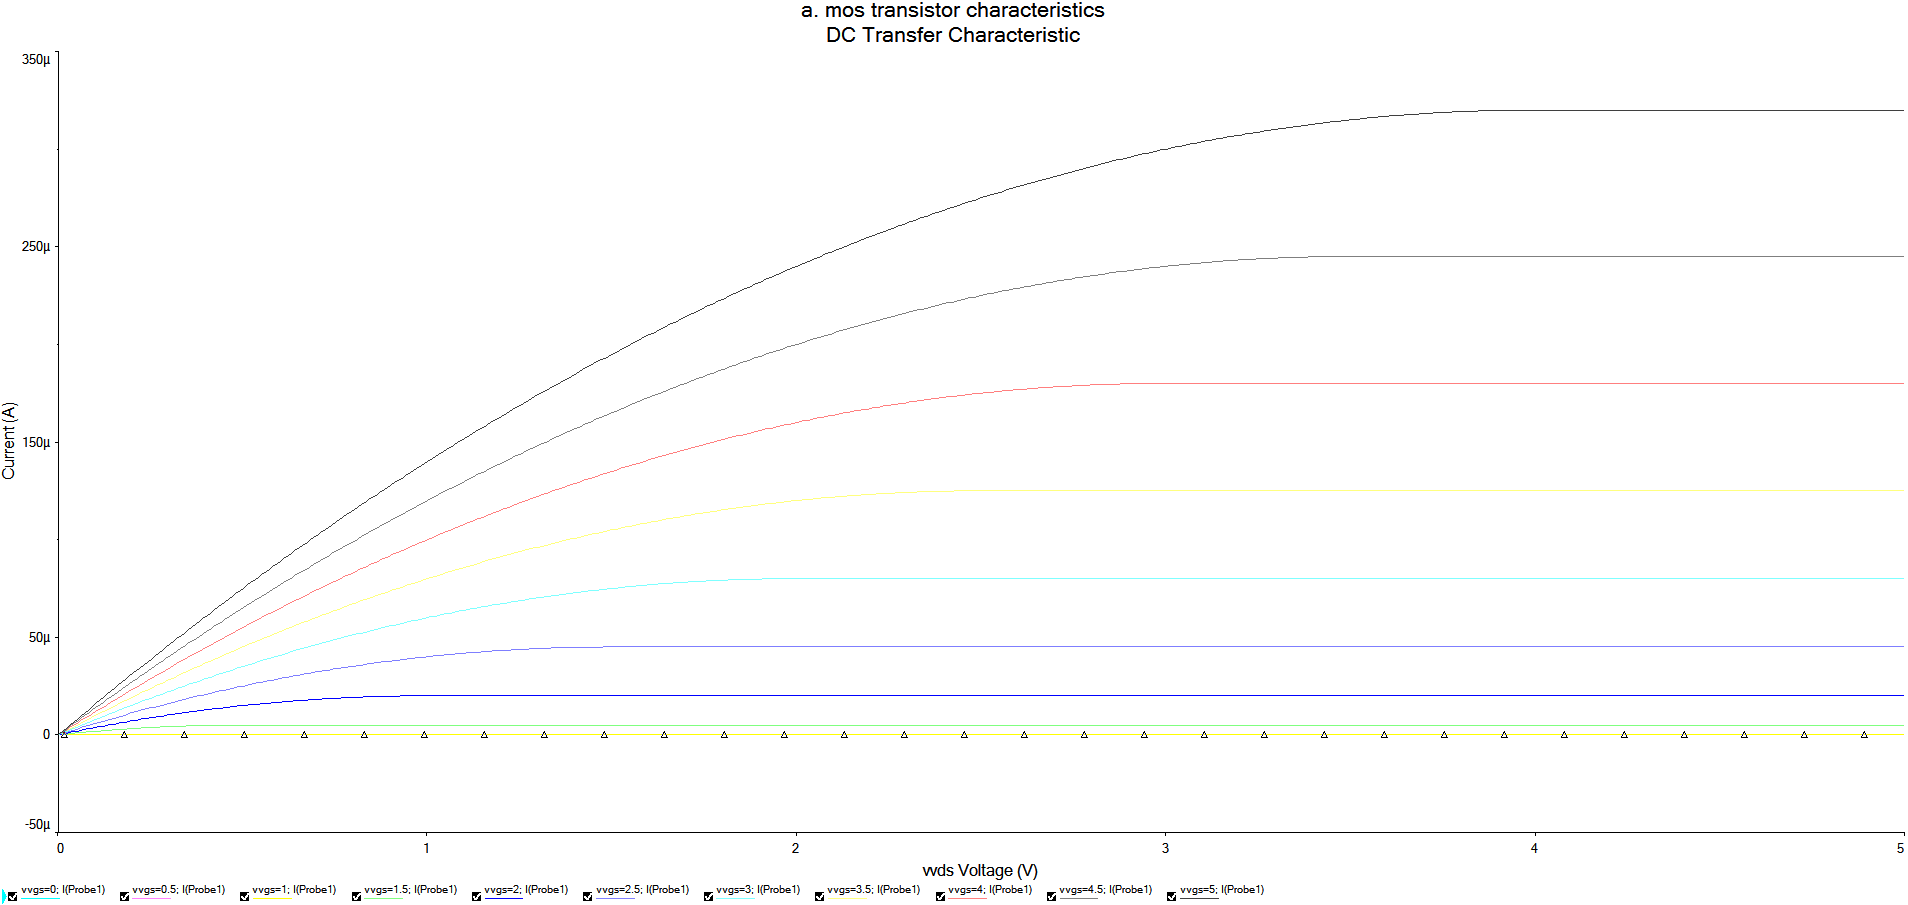
\includegraphics[width=1\textwidth]{a11.PNG}
\end{align*}

\begin{align*}
\centering
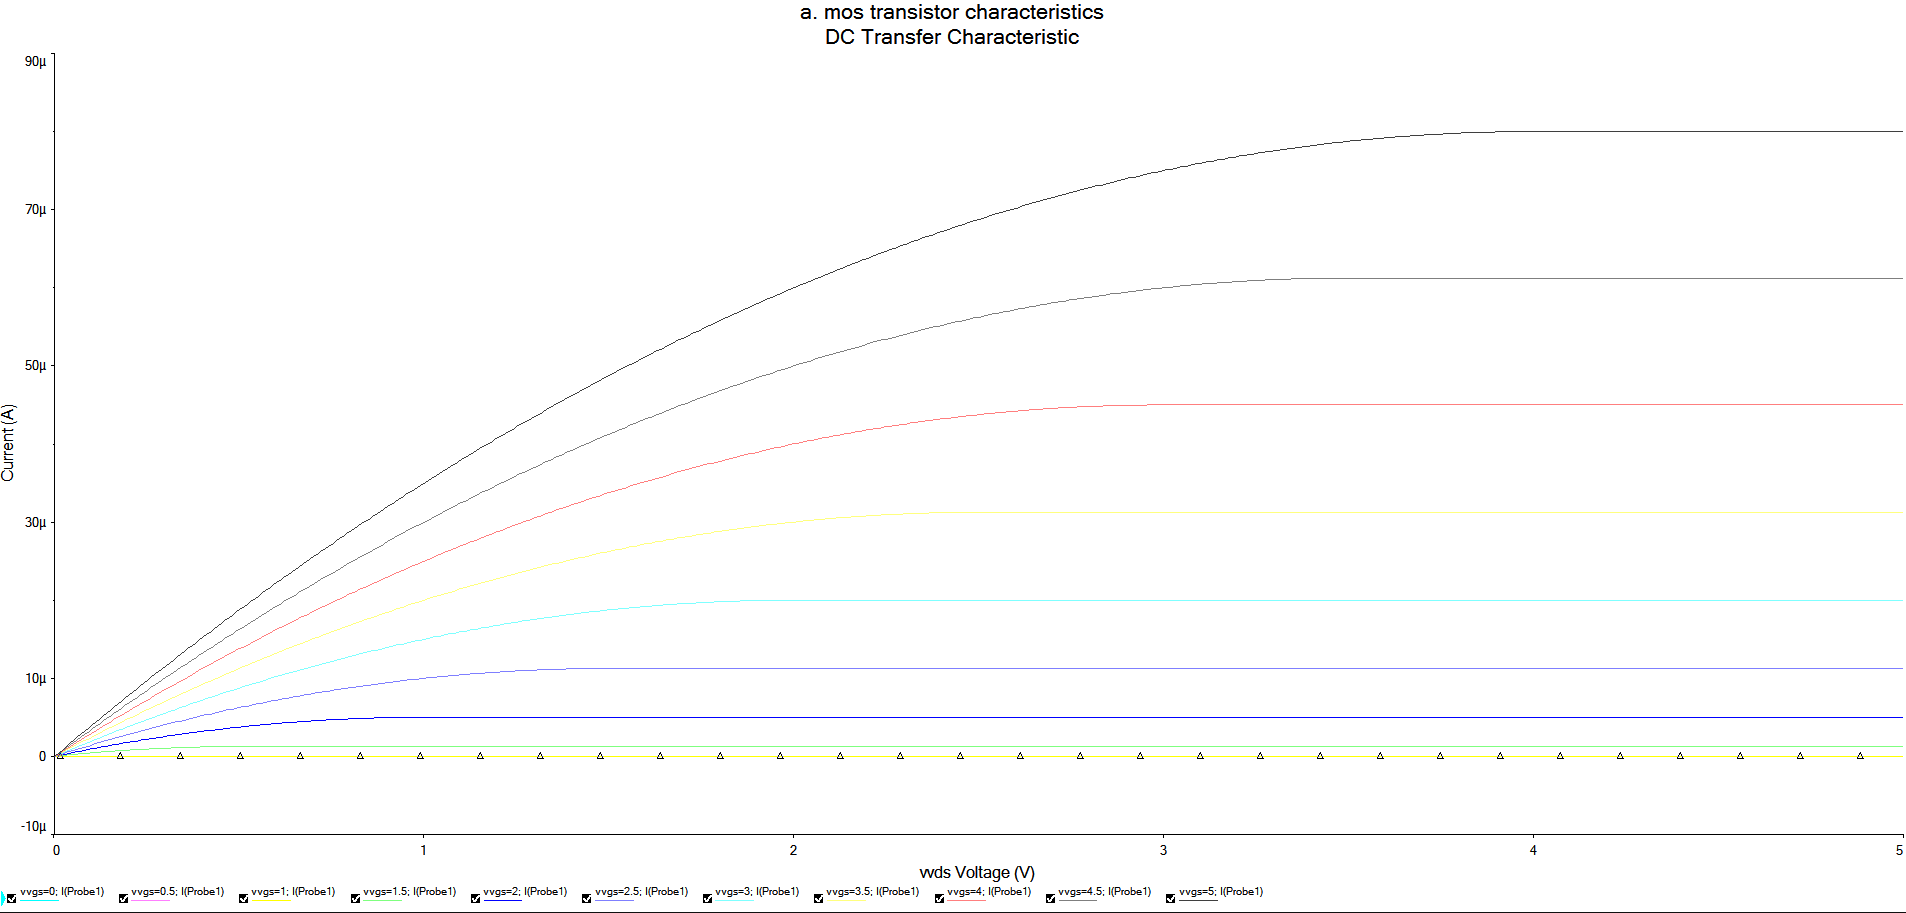
\includegraphics[width=1\textwidth]{a12.PNG}
\end{align*}
\subsection{Discussion}

\section{Resistively Loaded MOS Transistor Inverter}
\subsection{Procedure}
\begin{itemize}
\item Using the previously designed circuit, add the extra components to their respective positions by following the schematic provided.
\item When setting up a DC sweep, ensure that $V_{DS}$ is set to be source 1 instead of $V_{GS}$ where the probe is with respect to voltage, and not current.
\item When repeating the exercise, modify the resistor value $R_D$ to be 100k$\Omega$
\item Measure the logic values of $V_{IL MAX}$, $V_{IH MIN}$, $V_{OL}$, and $V_{OH}$ to be shown in the table below.
\end{itemize}
\subsection{Results}
Using the formula below, where $V_{GS}=V_{DD}$,
$$V_O=V_L=\left(V_{DD}-V_T+\frac{1}{2K_nR_D}\right)\pm\sqrt{\left(V_{DD}-V_T+\frac{1}{2K_nR_D}\right)^{2}-\frac{V_{DD}}{K_nR_D}}$$
We find that 100k$\Omega$ resistor has a $V_O$ of 7.44V or 0.305V, and the 25k$\Omega$ resistor has a $V_O$ of 8.87V or 1.127V.
\begin{table}[h]
\centering
\begin{tabular}{ll}
$V_{il max}$ & 1.51V \\
$V_{oh}$ & 5.05V \\
$V_{ih min}$ & 2.42V \\
$V_{ol}$ & 1.29V
\end{tabular}
\caption{25k$\Omega$ Resistor}
\end{table}

\begin{table}[h]
\centering
\begin{tabular}{ll}
$V_{il max}$ & 1.26V \\
$V_{oh}$ & 4.93V \\
$V_{ih min}$ & 1.17V \\
$V_{ol}$ & 645mV
\end{tabular}
\caption{100k$\Omega$ Resistor}
\end{table}

\begin{align*}
\centering
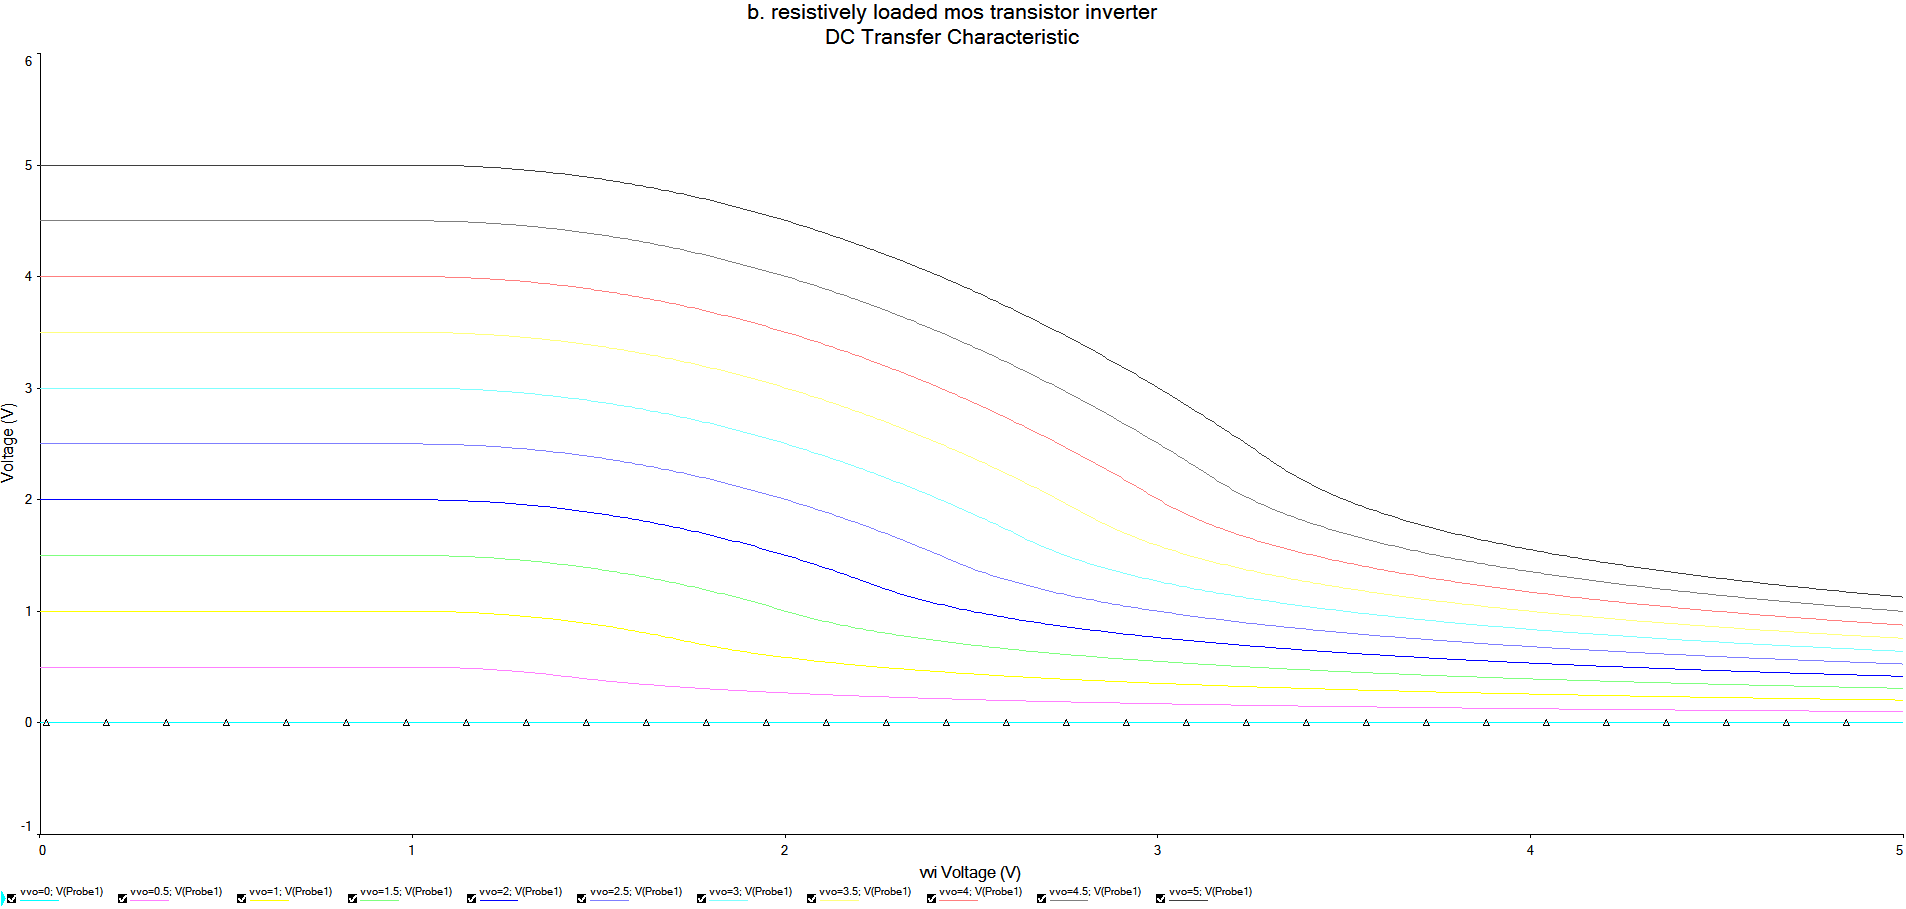
\includegraphics[width=1\textwidth]{b6.PNG}
\end{align*}

\begin{align*}
\centering
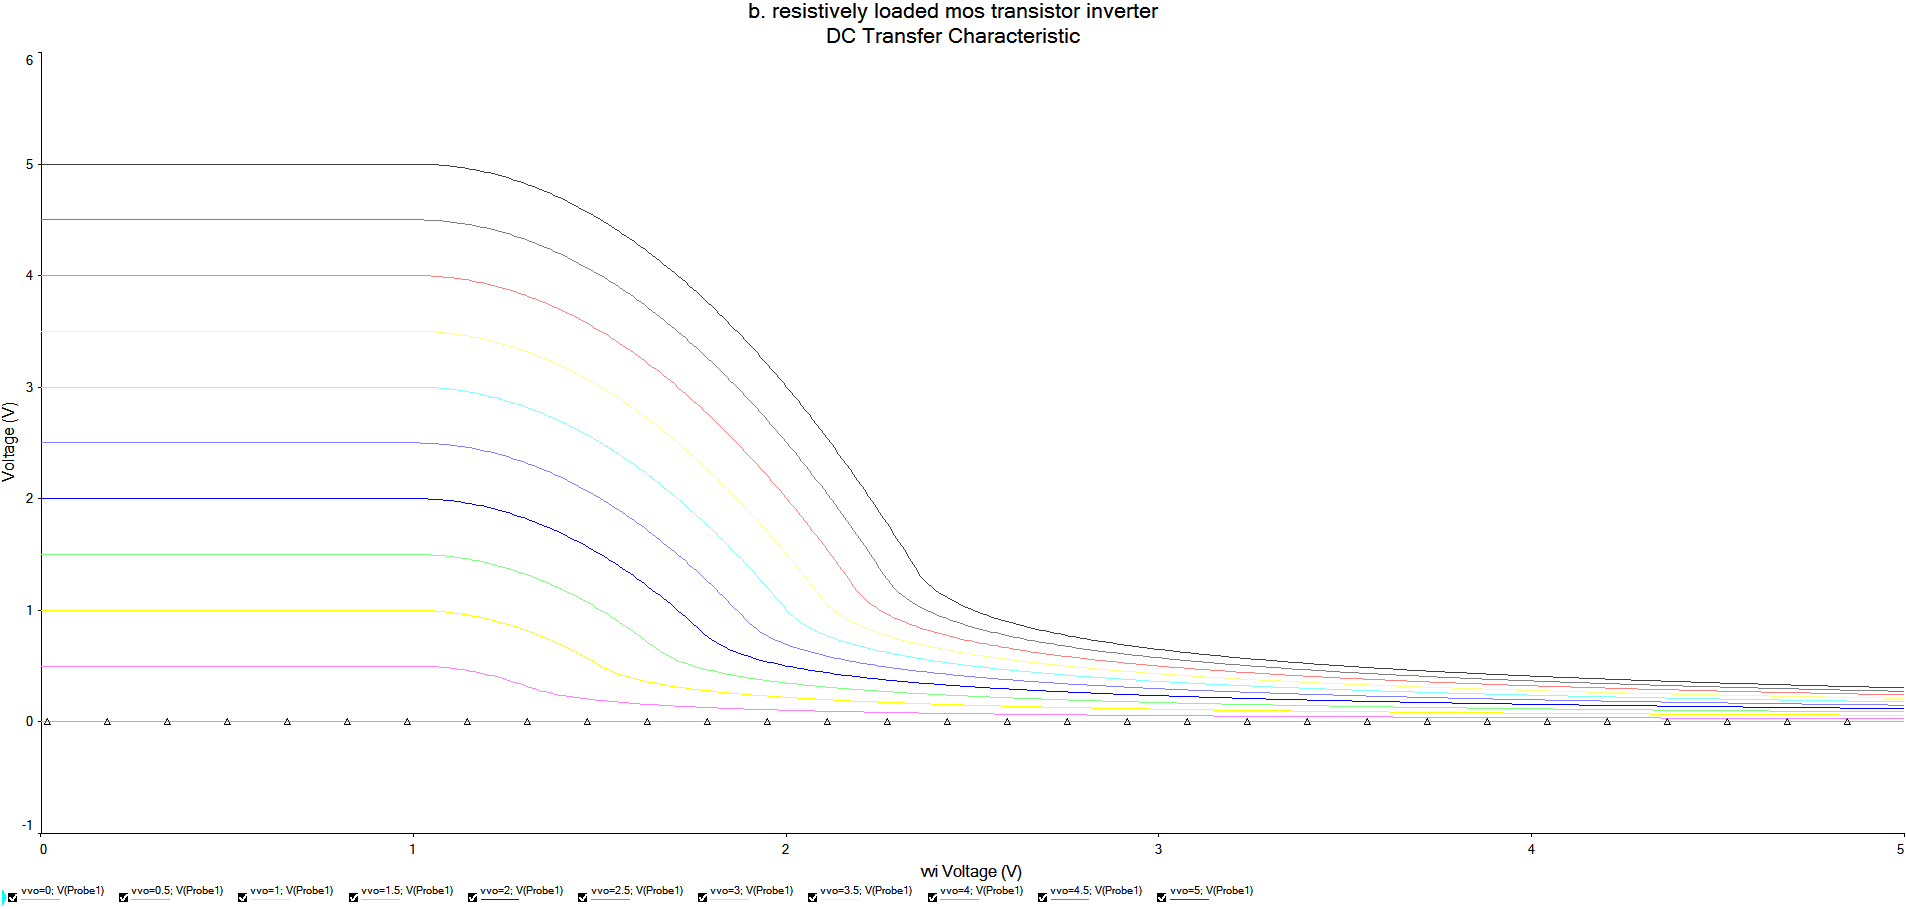
\includegraphics[width=1\textwidth]{b7.PNG}
\end{align*}
\subsection{Discussion}

\section{CMOS Inverter}
\subsection{Static Characteristics}
\subsubsection{Procedure}
\begin{itemize}
\item Create a new schematic and set up everything as shown in the diagram provided using the correct components.
\item Ensure the MOS transistors are facing the correct way, where in the case that they aren't, the can be flipped accordingly through right clicking on the component and selecting an option from the menu.
\item Set up a DC sweep for $V_{in}$ from 0-5V using an output probe of voltage as $V_O$.
\item Simulate the graph and use the cursors to obtain $V_{IL MAX}$, $V_{IH MIN}$, $V_{OL MAX}$, and $V_{OH MIN}$ at the points where the slope is tending to -1 in the appropriate regions of curvature.
\end{itemize}

\subsubsection{Results}

\begin{table}[h]
\centering
\begin{tabular}{ll}
$V_{il max}$ & 2.4V \\
$V_{ih min}$ & 2.6V \\
$V_{ol max}$ & 0.8V \\
$V_{oh min}$ & 4.2V
\end{tabular}
\caption{Static Characteristics}
\end{table}

\begin{align*}
\centering
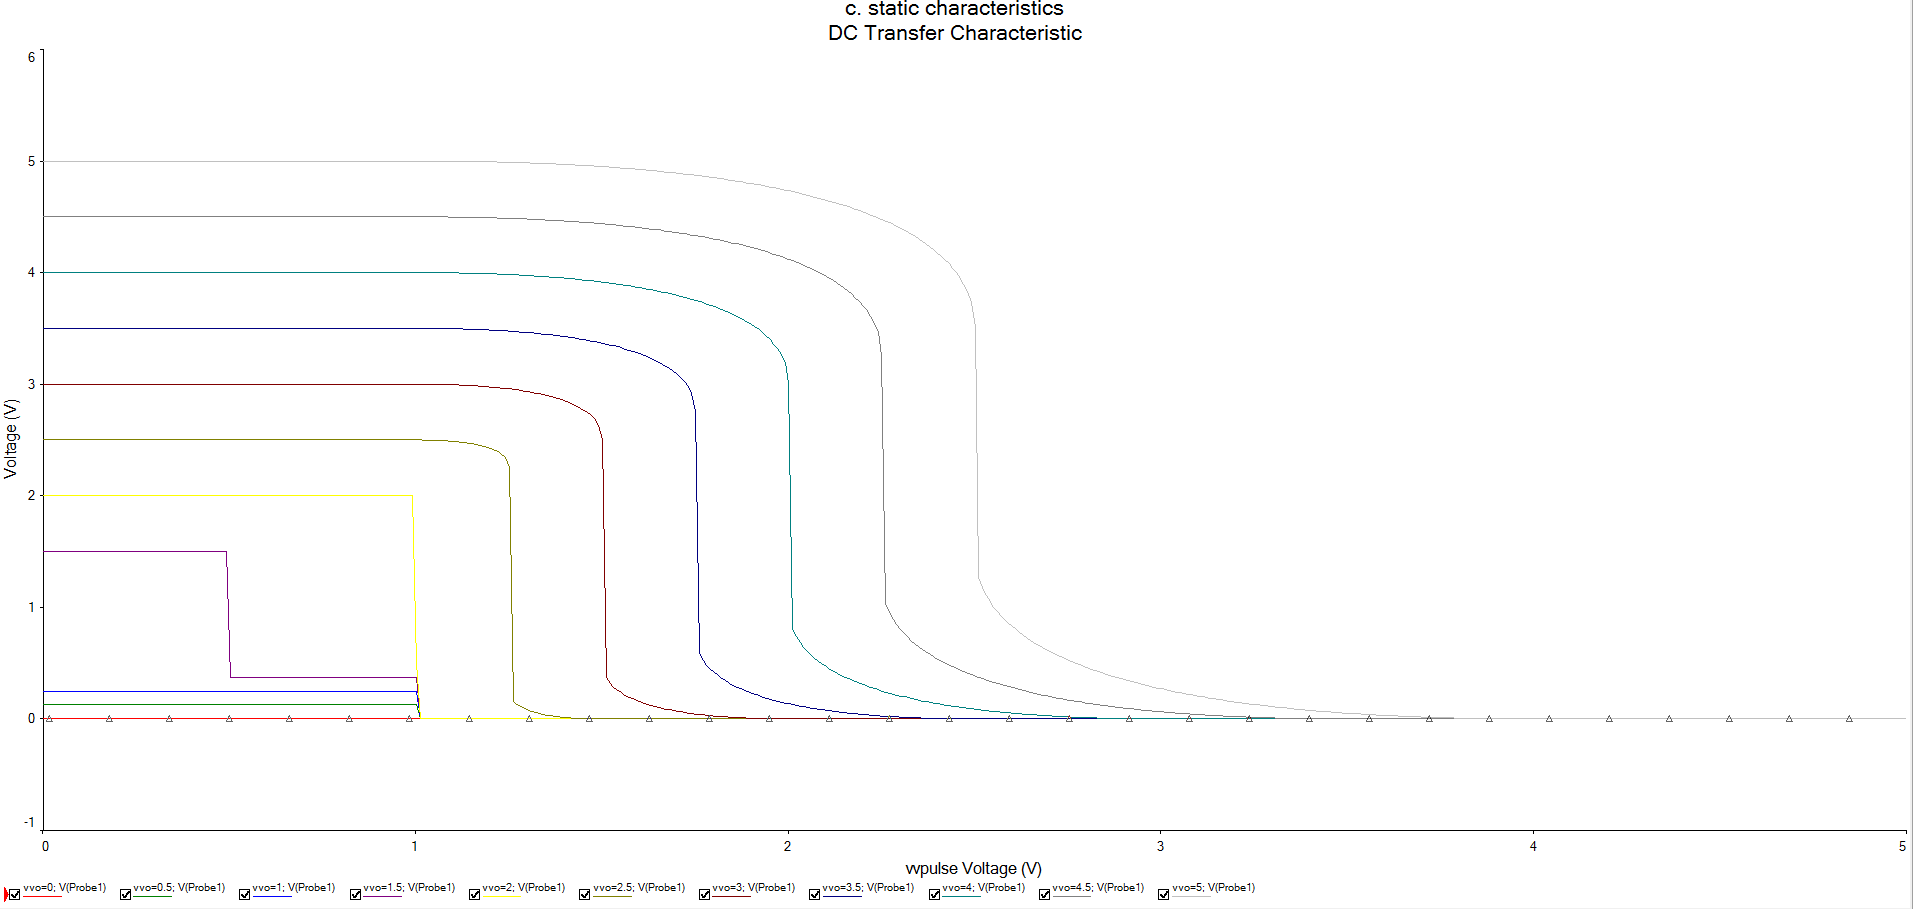
\includegraphics[width=1\textwidth]{c13.PNG}
\end{align*}
\subsubsection{Discussion}

\subsection{Dynamic Characteristics}
\subsubsection{Procedure}
\begin{itemize}
\item Using the schematic created in the previous part, modify the circuitry to include a capacitive dynamic condition in its configuration.
\item Using pulse voltage instead of a gate source this time, ensure the values from the image below are used.
\item Set up a transient analysis accordingly with a start time of 0, and end time of 2E-006, and a maximum time step of 4E-006.
\item Obtain the values for $t_{phl}$, $t_{plh}$, $t_f$, and $t_r$ as follows:
\begin{itemize}
\item $t_{phl}$: Input-output propagation delay at 50\% for a HI-LO transition
\item $t_{plh}$: Input-output propagation delay at 50\% for a LO-HI transition
\item $t_f$: Fall time over the 90\%-10\% HI-LO transition
\item $t_r$: Rise time over the 10\%-90\% LO-HI transition
\end{itemize}
\end{itemize}
\subsubsection{Results}

\begin{table}[h]
\centering
\begin{tabular}{ll}
$t_{PHL}$ & 0.07$\mu$s\\
$t_{PLH}$ & 81.1ns \\
$t_{f}$ & 187.1ns \\
$t_{r}$ & 1.1$\mu$s
\end{tabular}
\caption{Static Characteristics}
\end{table}

\begin{align*}
\centering
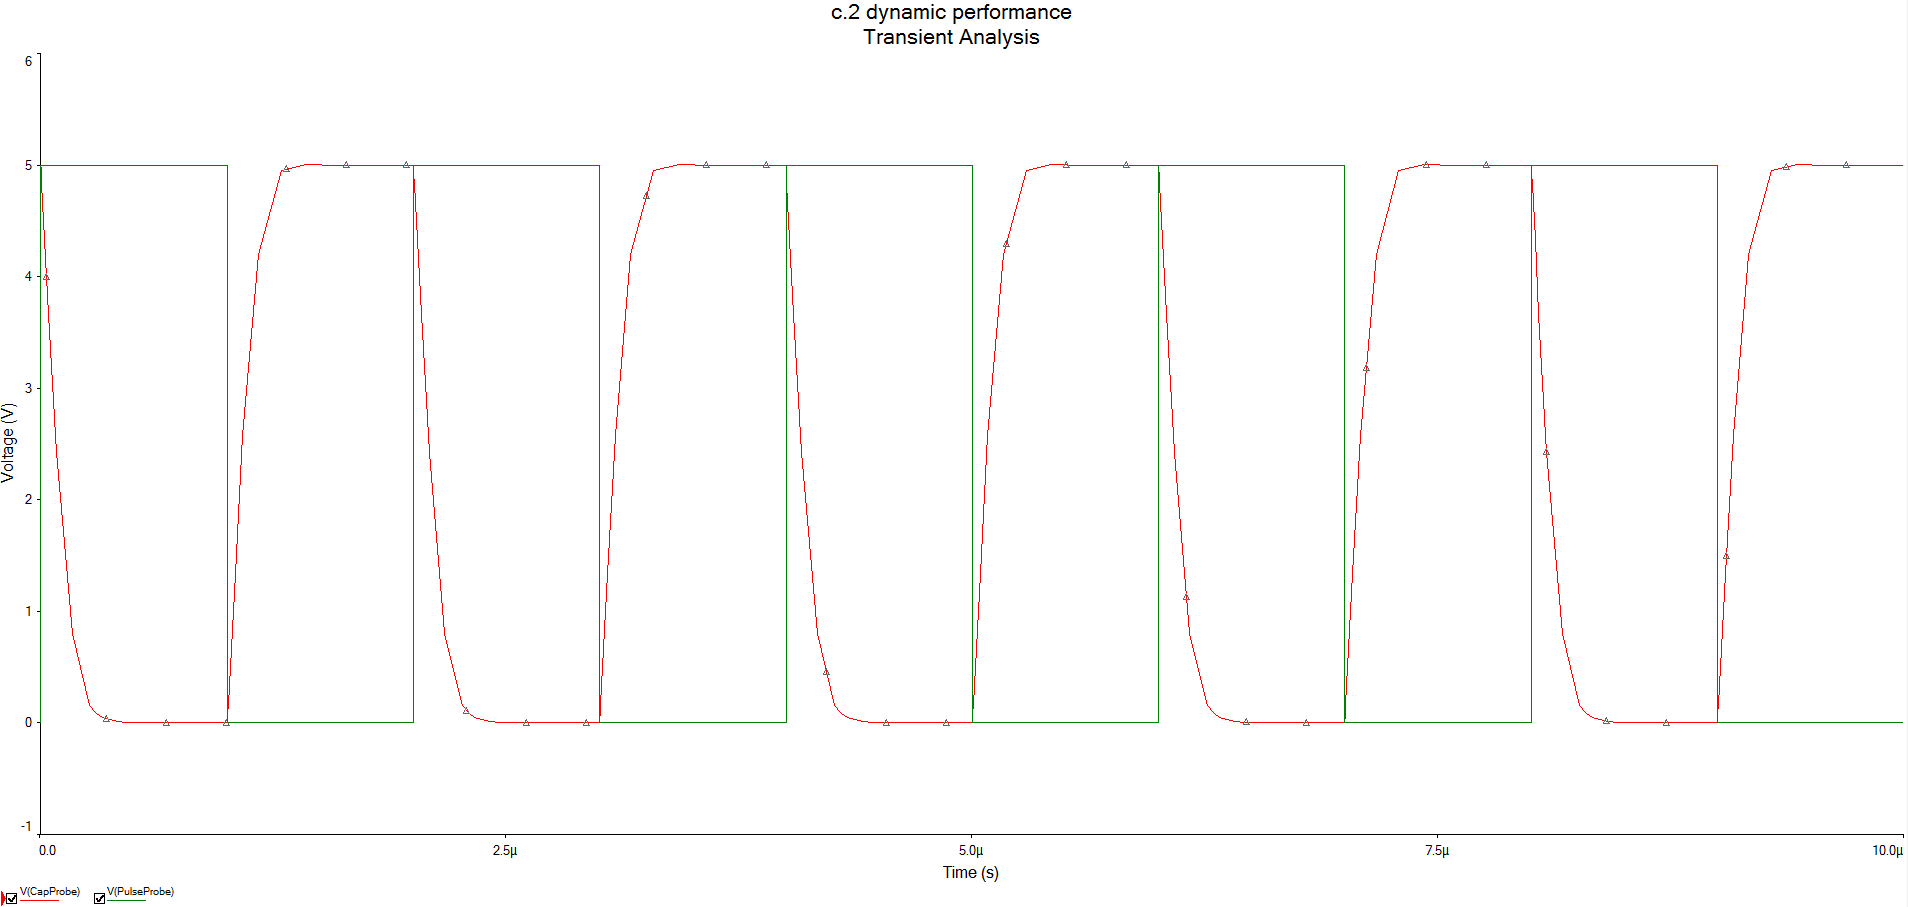
\includegraphics[width=1\textwidth]{c25.PNG}
\end{align*}
\subsubsection{Discussion}
\begin{itemize}
\item What are the limitations on the accuracy of your results?
\begin{itemize}
\item Human error and eye-balling results as an approximation were major contributions to error in results as the error wasn’t entirely standard overall and the results of approximation varied per person’s
judgement.
\end{itemize}
\item How do the values of parameters compare with those obtained in the lectures?
\begin{itemize}
\item The values obtained were somewhat similar to values in lectures. There are discrepancies in values though as those in lectures are always in an ideal and theoretical environment.
\end{itemize}
\item What are the advantages or disadvantages of circuit simulations such as the one carried out in the experiment?
\begin{itemize}
\item A great advantage of such a programme would be the ability to streamline and improve the design of the circuit without too much hassle and time involved in comparison to creating and testing it out
in real life. Although these are great advantages of Multisim, a disadvantage would be that this is always in an ideal world. As we live in a world that is not always ideal, there might be some environmental factors such as temperature that would tamper with actual values.
\end{itemize}
\item What are the benefits or drawbacks of circuit simulation and of MultiSim in general as applied to the design of electronic circuits?
\begin{itemize}
\item The simulator needs to be user friendly with the graphics. It needs to be able to work efficiently and calculate the values needed at the time needed. A large library of components needs to be available to use in the simulation. All modules are accurate and up to date with the current technology. 
\end{itemize}
\item What are the essential elements of good circuit simulation and simulators?
\begin{itemize}
\item The simulator needs to be user friendly with the graphics. It needs to be able to work efficiently and calculate the values needed at the time needed. A large library of components needs to be available to use in the simulation. All modules are accurate and up to date with the current technology
\end{itemize}
\item What is the roll of the Electronic Engineer in this regard?\begin{itemize}
\item The role in this regard would be to understand how to use the software package in an efficient and educated manner. In order to do this however, a strong understanding of circuitry is required and the limits of the circuit itself.
\end{itemize}
\end {itemize}
\section{Bibliography}
\begin{thebibliography}{3}
\bibitem{streetmanb}
  Ben G. Streetman \& Sanjay Kumar Banerjee,
  \emph{Solid State Electronic Devices, 6th edition},
  Prentice Hall (2006),
  Pages 154-388.
\end{thebibliography}
\end{document}
